\documentclass{article}
\usepackage[margin=1in]{geometry}
\usepackage[utf8]{inputenc}
\usepackage{listings}
\usepackage{hyperref}
\usepackage{graphicx}
\usepackage{float}
\usepackage{xcolor}

\definecolor{codegreen}{rgb}{0,0.6,0}
\definecolor{codegray}{rgb}{0.5,0.5,0.5}
\definecolor{codepurple}{rgb}{0.58,0,0.82}
\definecolor{backcolour}{rgb}{0.95,0.95,0.92}

\lstdefinestyle{mystyle}{
    backgroundcolor=\color{backcolour},   
    commentstyle=\color{codegreen},
    keywordstyle=\color{magenta},
    numberstyle=\tiny\color{codegray},
    stringstyle=\color{codepurple},
    basicstyle=\ttfamily\footnotesize,
    breakatwhitespace=false,         
    breaklines=true,                 
    captionpos=b,                    
    keepspaces=true,                 
    numbers=left,                    
    numbersep=5pt,                  
    showspaces=false,                
    showstringspaces=false,
    showtabs=false,                  
    tabsize=2
}

\lstset{style=mystyle}

\title{ECE 4310\\Operating Systems for Embedded Application\\\,\\Project 2}
\author{Choi Tim Antony Yung}
\begin{document}
\maketitle

\thispagestyle{empty}
\setcounter{page}{0}

\newpage

\section{\texttt{vmstat} and \texttt{free}}

\subsection{\texttt{vmstat}}

\begin{figure}[H]

  \caption{Output of \texttt{vmstat}}
  \centering
  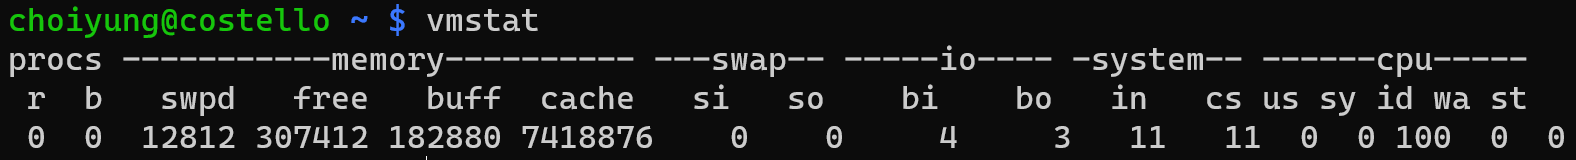
\includegraphics[width=0.75\textwidth]{ECE4310_proj2_vmstat.png}
\end{figure}

\begin{figure}[H]
  \caption{Output of \texttt{man vmstat}}
  \centering
  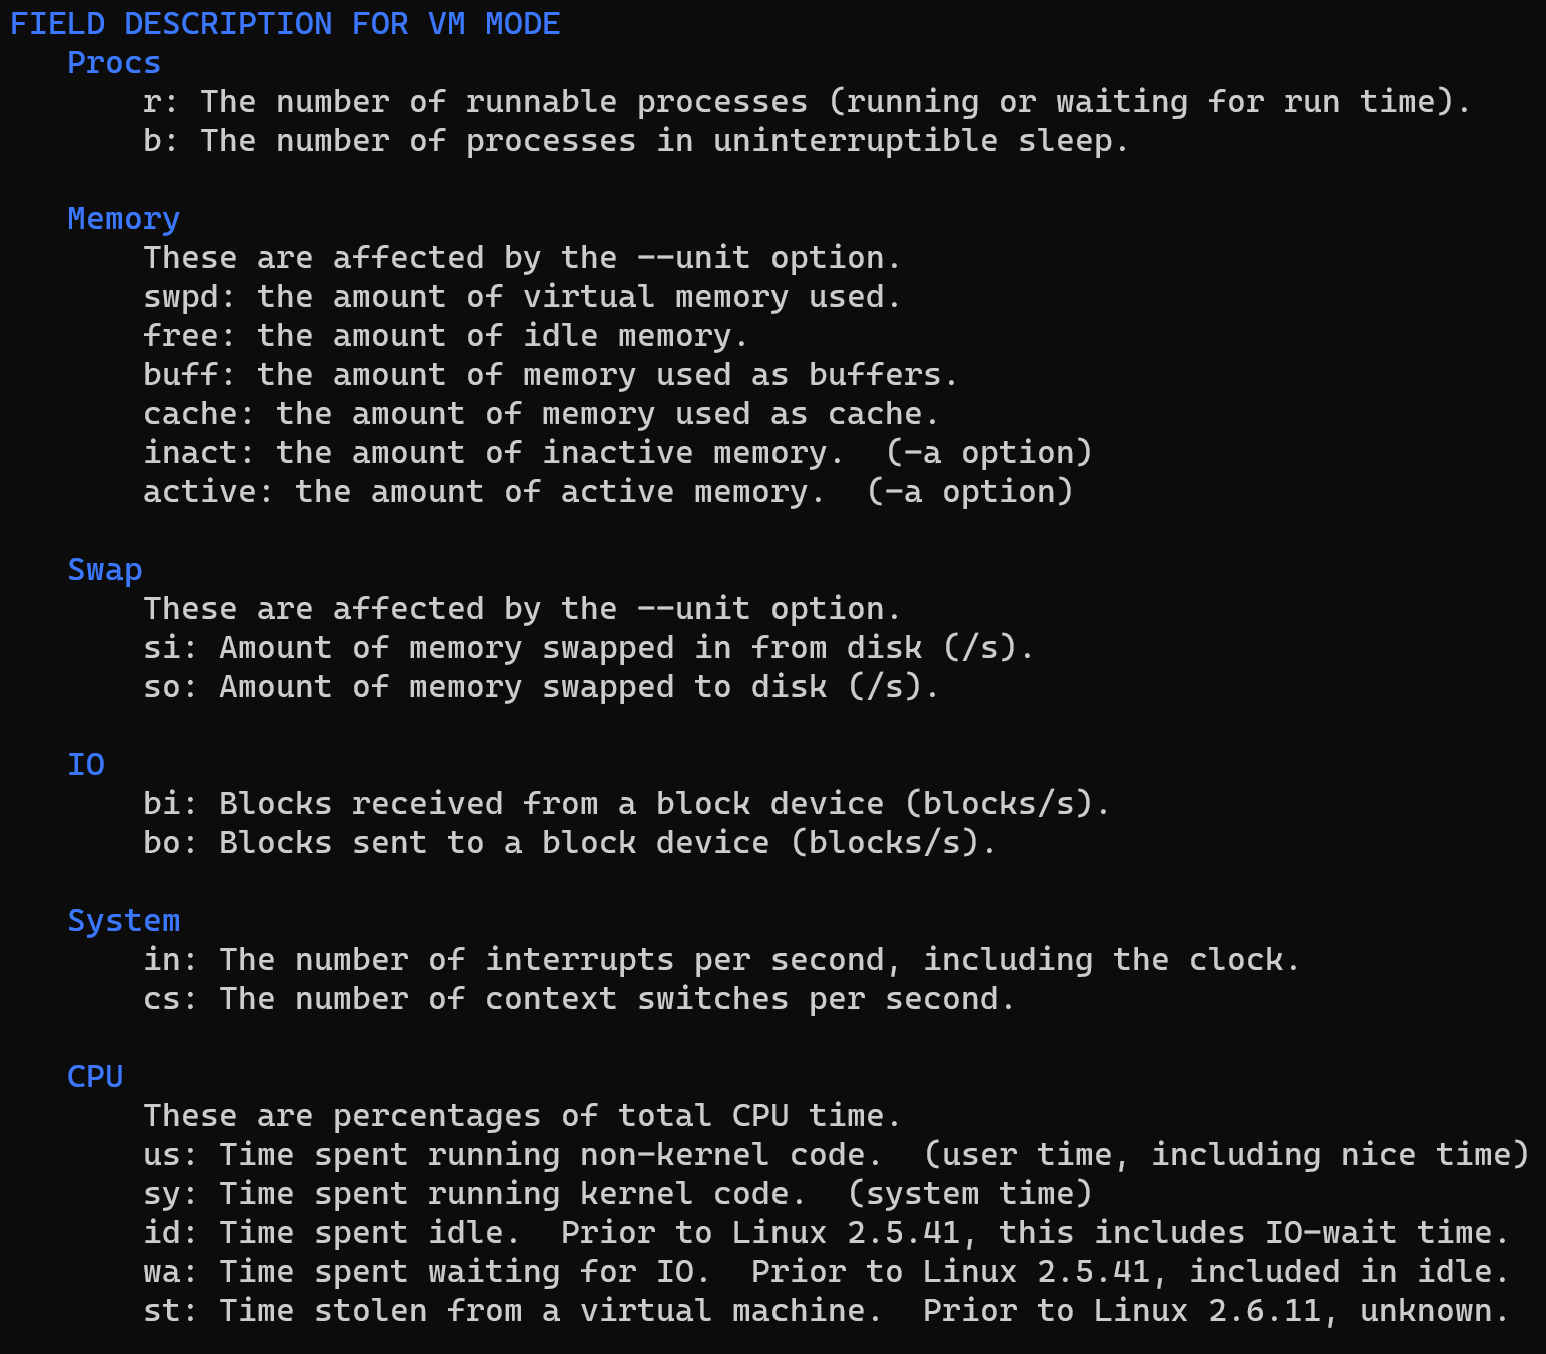
\includegraphics[width=0.75\textwidth]{ECE4310_proj2_vmstat_man.png}
\end{figure}

According to the \texttt{man} page:
\begin{itemize}
  \item r indicate there are currently no processes running or waiting;
  \item b indicate there are currently no processes in uninterruptible sleep;
  \item swpd is the amount of virtual memory/swap memory/pagefile/backing store used;
  \item free is the amount of physical memory not in use;
  \item buff is the amount of physical memory used as buffers;
  \item cache is the amount of physical memory used as caches;
  \item si is the amount of swapping/paging in per second, indicating if some page was swapped back to physical memory;
  \item so is the amount of swapping/paging out per second, indicating if some page was swapped to disk to free frames;
  \item bi is the amount of blocks received from a block device, i.e. input from some hardware devices
  \item bo is the amount of blocks sent to a block device, i.e. output to some hardware devices
  \item in is the number of interrupts per second
  \item cs is the number of context switches per second
  \item us is the percentage of CPU time running non-kernel code
  \item sy is the percentage of CPU time running kernel code
  \item id is the percentage of CPU time being idle
  \item wa is the percentage of CPU time waiting for IO
  \item st is the percentage of CPU time stolen from virtual machine
\end{itemize}

From the \texttt{vmstat} output, it can be determined that no user space processes are currently running or sleeping; 
12812B of backing store is in use; 307412B of physical memory is not in use; 182880B of physical memory is used as buffer; 
7418876B of physical memory is used as cache; There are no paging in or paging out, meaning there are enough physical memory for processes running;
Some blocks are being transferred indicating accesses to block devices (usually mass storage); Multiple processes are running, hence the interrupts and context switching; 
and CPU spent almost all its time being idle. 


\subsection{\texttt{free}}

\begin{figure}[H]

  \caption{Output of \texttt{free}}
  \centering
  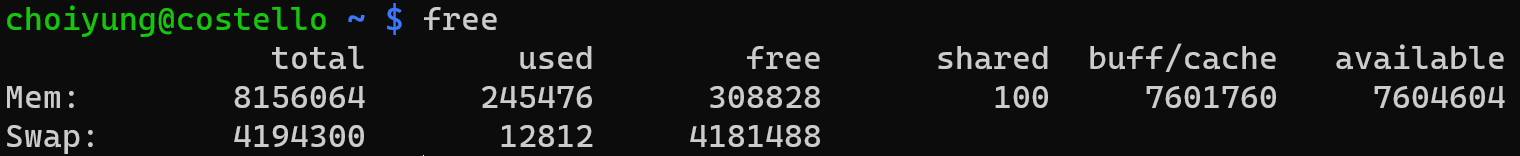
\includegraphics[width=0.75\textwidth]{ECE4310_proj2_free.png}
\end{figure}

\begin{figure}[H]
  \caption{Output of \texttt{man free}}
  \centering
  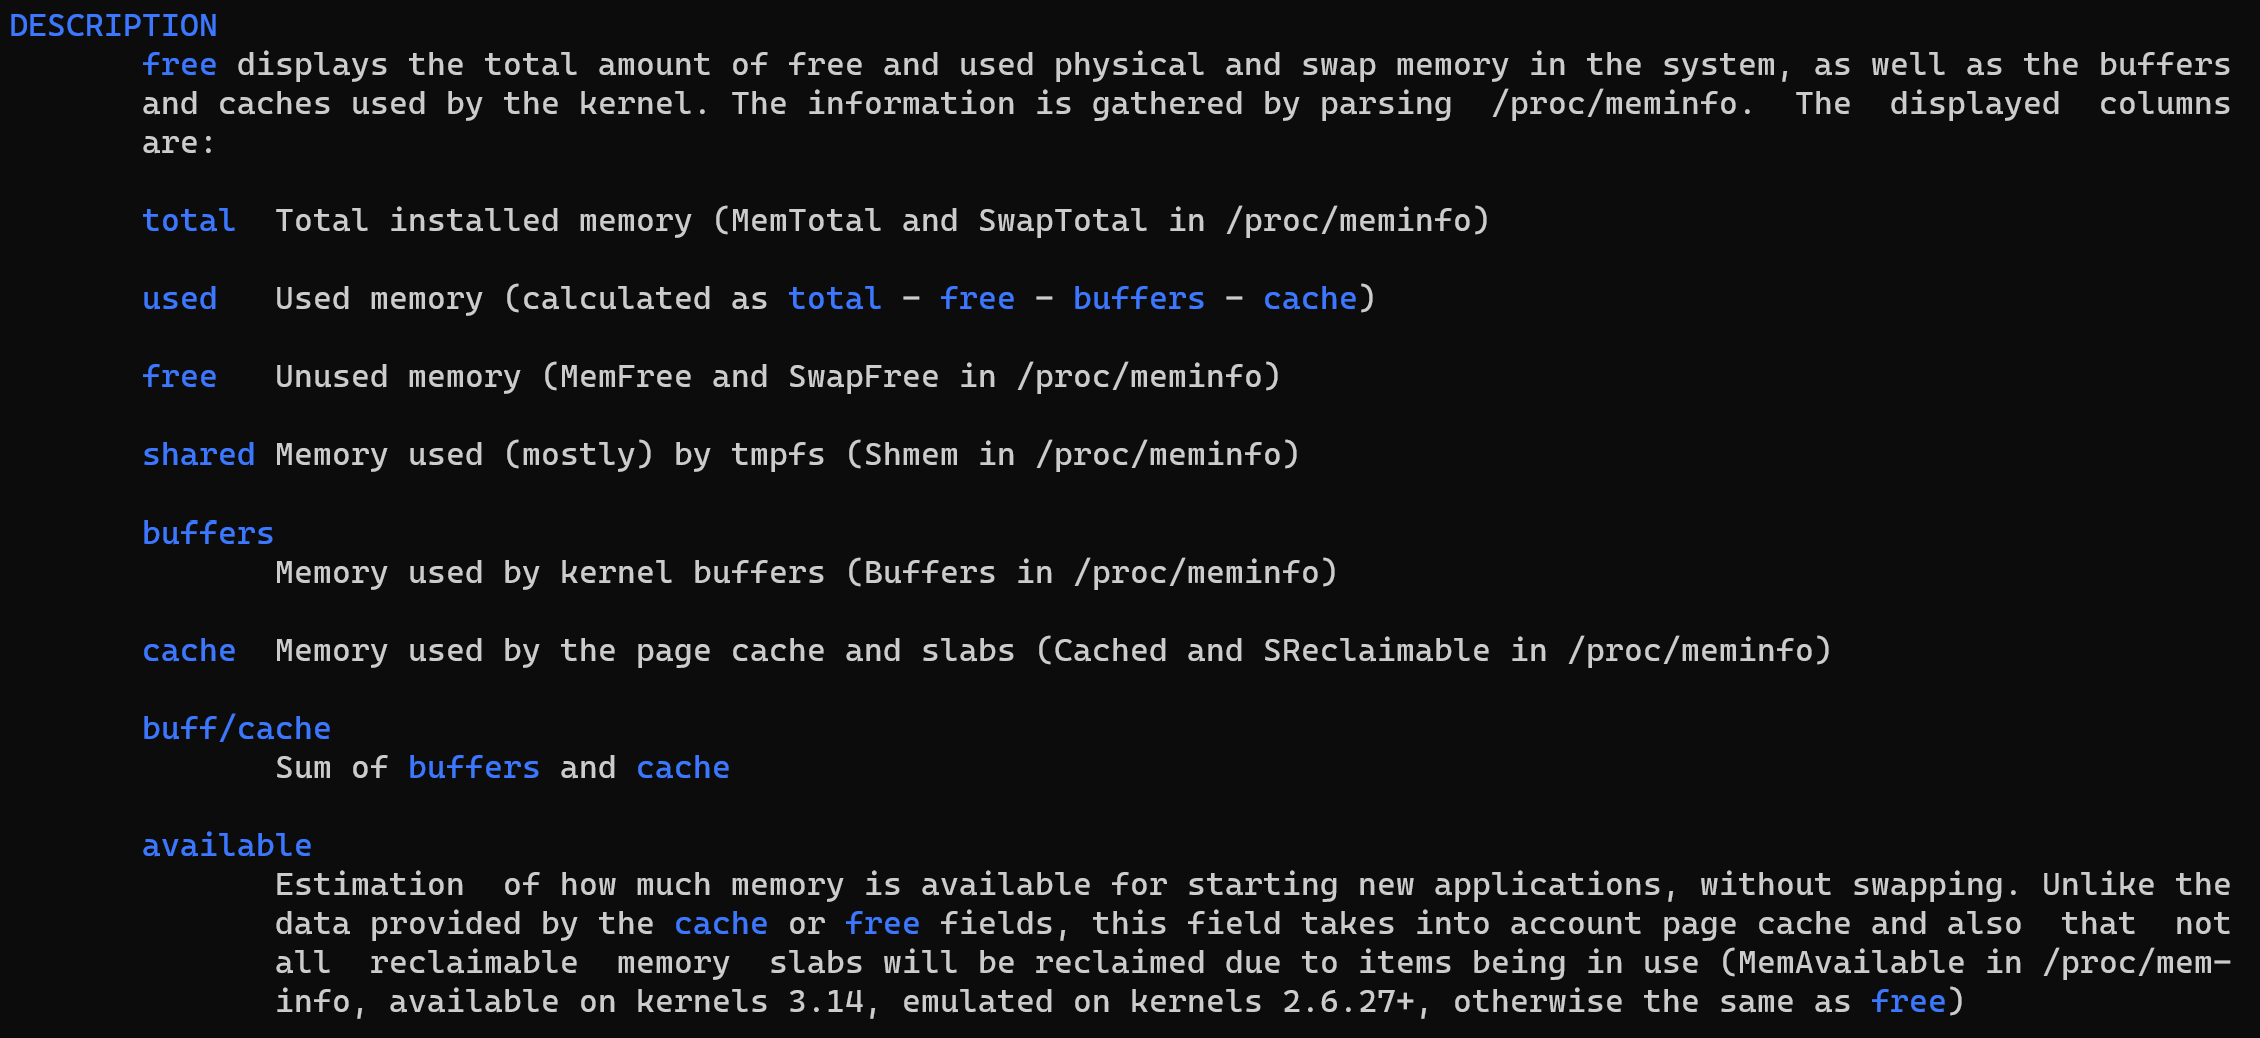
\includegraphics[width=0.75\textwidth]{ECE4310_proj2_free_man.png}
\end{figure}

From the \texttt{free} output, it can be determined that the system have a total of 8156064B of physical memory, 
245476B are allocated to processes, 308828B of physical memory are not used, 100B seems to be used mostly by tmpfs to provide a fast access file system, 
7601760B are used as buffers or cache, and 7604604B can be allocated to new process. 
Also, there are a total of 4194300B of mass storage space allocated for backing store, 12812B of them are used and 4181488B are not.

\section{Paging Simulation}
\subsection*{Code}
\lstinputlisting[language=C]{ECE4310_proj2_2.c}
\begin{figure}[H]

  \caption{Output of the code}
  \centering
  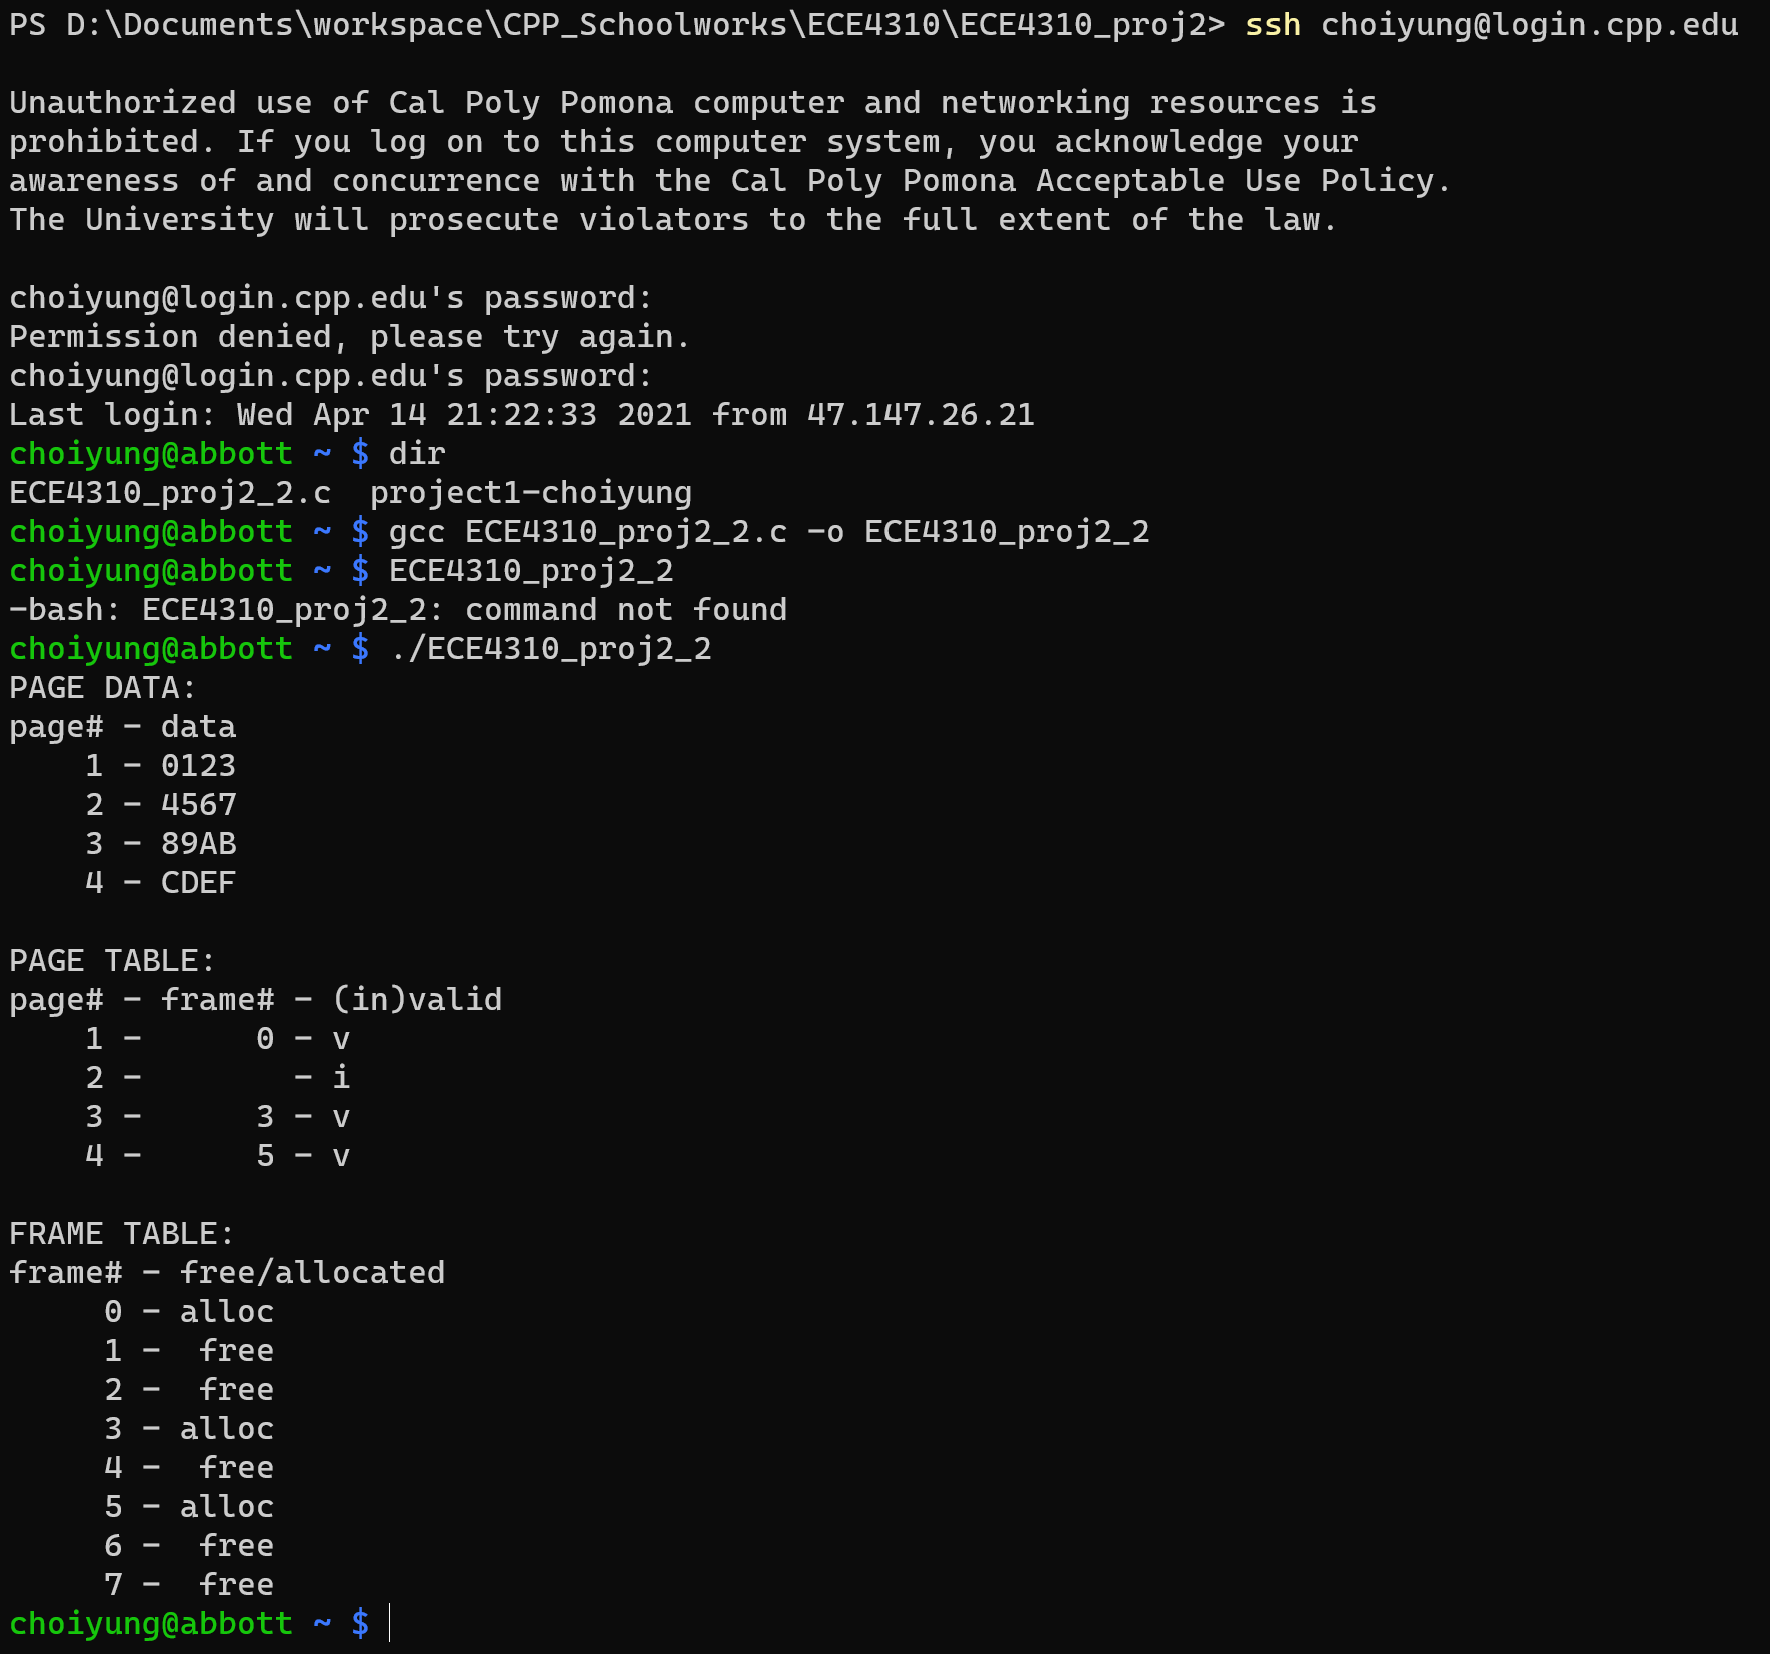
\includegraphics[width=0.75\textwidth]{ECE4310_proj2_2_abbott.png}
\end{figure}

\end{document}
